% AMSC-HAR project report
% Compile: pdflatex main.tex && pdflatex main.tex
\documentclass[11pt,a4paper]{article}

\usepackage[T1]{fontenc}
\usepackage[utf8]{inputenc}
\usepackage{lmodern}
\usepackage[margin=2.2cm]{geometry}
\usepackage{amsmath,amssymb,amsthm}
\usepackage{booktabs}
\usepackage{tabularx}
\usepackage{multirow}
\usepackage{graphicx}
\usepackage{tikz}
\usetikzlibrary{arrows.meta,positioning,fit,calc,chains}
\usepackage{xcolor}
\usepackage{listings}
\usepackage{hyperref}
\usepackage{enumitem}
\usepackage{caption}
\usepackage{setspace}
\usepackage{titlesec}

\hypersetup{
  colorlinks=true,
  linkcolor=black,
  citecolor=black,
  urlcolor=blue!50!black
}

\definecolor{codebg}{RGB}{247,247,248}
\lstset{
  basicstyle=\ttfamily\footnotesize,
  backgroundcolor=\color{codebg},
  frame=single,
  framerule=0.3pt,
  rulecolor=\color{black!20},
  breaklines=true,
  columns=fullflexible,
  keepspaces=true,
  xleftmargin=0.4em,
  xrightmargin=0.4em,
  aboveskip=0.7em,
  belowskip=0.7em
}

\titleformat{\section}{\large\bfseries}{\thesection}{0.6em}{}
\titleformat{\subsection}{\normalsize\bfseries}{\thesubsection}{0.5em}{}
\setlist[itemize]{leftmargin=1.4em,itemsep=0.15em,topsep=0.25em}
\setlist[enumerate]{leftmargin=1.4em,itemsep=0.15em,topsep=0.25em}
\setlength{\parskip}{0.35em}
\setlength{\parindent}{0pt}
\onehalfspacing

\title{\textbf{Human Action Recognition with a from-scratch\\
C++23 Video CNN}\\[0.4em]
\large AMSC Project Report}
\author{AMSC-HAR\\
Politecnico di Milano\\
Advanced Methods for Scientific Computing}
\date{\today}

\begin{document}
\maketitle
\vspace{-1.2em}

\begin{abstract}
This report describes \textbf{AMSC-HAR}, a header-only C++23 library and
command-line trainer for video-based human action recognition.
Unlike typical student projects that wrap PyTorch or TensorFlow, the system
implements tensors, layers, automatic-style reverse-mode gradients, SGD,
checkpointing, video decoding, and optional CUDA kernels from scratch.
The model is a compact VideoCNN: a shared 2D convolutional backbone over
sampled RGB frames, a residual temporal 1D convolution, learnable temporal
attention pooling, and a linear classifier.
On the UCF11 (YouTube Action) dataset the default recipe uses $64\times 64$
frames, $T=8$ uniformly sampled time steps, and about $5.9\times 10^5$
trainable parameters.
A held-out inference check with the released best checkpoint
\texttt{ucf11\_videocnnBest.harw} classified $8/10$ randomly drawn clips
correctly (80\%), with several classes predicted at $>95\%$ confidence.
The same codebase also targets UCF101 official splits.
This document covers design goals, software architecture, the mathematical
model, the data pipeline, training, the CUDA backend, and experimental
results.
\end{abstract}

\tableofcontents
\vspace{0.6em}

%----------------------------------------------------------------------
\section{Introduction}
\label{sec:intro}

Human action recognition (HAR) from video is a standard benchmark for
spatio-temporal representation learning~\cite{soomro2012ucf101,liu2009ucf11}.
A short clip must be mapped to one of a fixed set of action classes
(e.g.\ \emph{diving}, \emph{tennis swing}, \emph{walking a dog}).
The academic community usually solves this with large 3D CNNs or
transformer video models trained in Python frameworks.
Those stacks hide the linear algebra, memory layout, and gradient bookkeeping
that a scientific-computing course is meant to expose.

AMSC-HAR takes the opposite route.
The project is a \emph{complete} recognition pipeline written in modern C++:
\begin{itemize}
  \item a generic \texttt{Tensor<T>} with CPU storage and optional
        CUDA Unified Memory;
  \item layers with explicit \texttt{forward}/\texttt{backward} (Conv2D,
        BatchNorm2D, ReLU, pooling, Dropout, Linear, TemporalConv1D,
        temporal attention);
  \item SGD with momentum and $\ell_2$ weight decay;
  \item softmax cross-entropy;
  \item OpenCV (or FFmpeg) video decoding, a binary clip cache, and
        train-time augmentation;
  \item a custom checkpoint format \texttt{.harw};
  \item a single executable \texttt{har\_cnn} for smoke tests, training,
        prediction, and split evaluation.
\end{itemize}

\paragraph{Contributions.}
(1)~A compact, auditable VideoCNN that stays under 0.6M parameters while
remaining strong on UCF11.
(2)~A dual CPU/CUDA path so the same headers train on a laptop or a GPU.
(3)~An end-to-end data path (decode $\to$ cache $\to$ temporal sample
$\to$ batch) that makes repeated epochs practical.
(4)~Reproducible CLI defaults (seed 42, $80/10/10$ UCF11 split) and a
self-describing weight file that stores image size, clip length, and class
names.

\paragraph{Report outline.}
Section~\ref{sec:bg} recalls HAR and the datasets.
Section~\ref{sec:arch} presents the repository layout and CLI.
Section~\ref{sec:tensor} describes tensors and layers.
Section~\ref{sec:model} specifies VideoCNN.
Section~\ref{sec:data} covers decoding and augmentation.
Section~\ref{sec:train} details the training loop.
Section~\ref{sec:cuda} summarises CUDA kernels.
Section~\ref{sec:exp} reports experiments.
Section~\ref{sec:conc} concludes.

%----------------------------------------------------------------------
\section{Background and problem statement}
\label{sec:bg}

\subsection{Video action recognition}

A video is a tensor $X\in\mathbb{R}^{T\times C\times H\times W}$.
The classifier produces logits $z\in\mathbb{R}^{K}$ and a predicted class
$\hat{y}=\arg\max_k z_k$.
Early HAR used hand-crafted descriptors (HOG, HOF, dense
trajectories)~\cite{wang2013dt}.
Two-stream networks~\cite{simonyan2014twostream} combined RGB appearance
with optical flow.
3D CNNs such as C3D~\cite{tran2015c3d} and I3D~\cite{carreira2017i3d}
convolve jointly over space and time.
Recent work uses space--time transformers, which are accurate but expensive.

AMSC-HAR uses a cheaper and more transparent design:
\emph{2D CNN on each frame}, then a \emph{1D temporal mixer} and
\emph{attention pooling}.
This is close in spirit to TSN / TRN-style late temporal
aggregation~\cite{wang2016tsn}, but the temporal conv and attention are
trained jointly with the backbone.

\subsection{Datasets}

\paragraph{UCF11} (YouTube Action)~\cite{liu2009ucf11} contains 11 sport and
daily actions, originally published as MPEG clips crawled from YouTube.
This project uses the updated \texttt{UCF11\_updated\_mpg} release
(1600 clips after scanning the extracted tree).
UCF11 has no official train/test list, so the loader applies a
class-stratified shuffle (seed 42) with default ratios
$80\%$ train / $10\%$ val / $10\%$ test.

\paragraph{UCF101}~\cite{soomro2012ucf101} has 101 classes and three official
recognition splits.
The same VideoCNN is reused; only the classifier width and the split
reader change.

Table~\ref{tab:ucf11} lists the UCF11 classes as stored in the best
checkpoint (alphabetical folder names).

\begin{table}[t]
\centering
\caption{UCF11 classes and clip counts in \texttt{data/UCF11\_updated\_mpg}.}
\label{tab:ucf11}
\small
\begin{tabular}{@{}lrlr@{}}
\toprule
Class & Clips & Class & Clips \\
\midrule
basketball            & 141 & soccer\_juggling      & 156 \\
biking                & 145 & swing                 & 137 \\
diving                & 156 & tennis\_swing         & 167 \\
golf\_swing           & 142 & trampoline\_jumping   & 119 \\
horse\_riding         & 198 & volleyball\_spiking   & 116 \\
                      &     & walking               & 123 \\
\midrule
\multicolumn{3}{@{}l}{Total} & 1600 \\
\bottomrule
\end{tabular}
\end{table}

\subsection{Design constraints}

The course setting imposes constraints that shaped every API choice:
\begin{enumerate}
  \item \textbf{No deep-learning runtime.} Gradients, convolution, and
        BatchNorm are written out, not imported.
  \item \textbf{C++23.} Concepts, \texttt{std::format}, ranges, and
        \texttt{std::filesystem} keep the headers short.
  \item \textbf{Optional GPU.} CUDA 13 kernels exist, but CPU paths remain
        correct and are the fallback used in this report's inference run.
  \item \textbf{Memory budget.} Activations of a $112\times 112$, $T=16$
        batch are capped so a 12\,GB card does not oversubscribe Unified
        Memory.
\end{enumerate}

%----------------------------------------------------------------------
\section{Software architecture}
\label{sec:arch}

The repository is organised as a small scientific library plus one
executable (Figure~\ref{fig:repo}).

\begin{figure}[t]
\centering
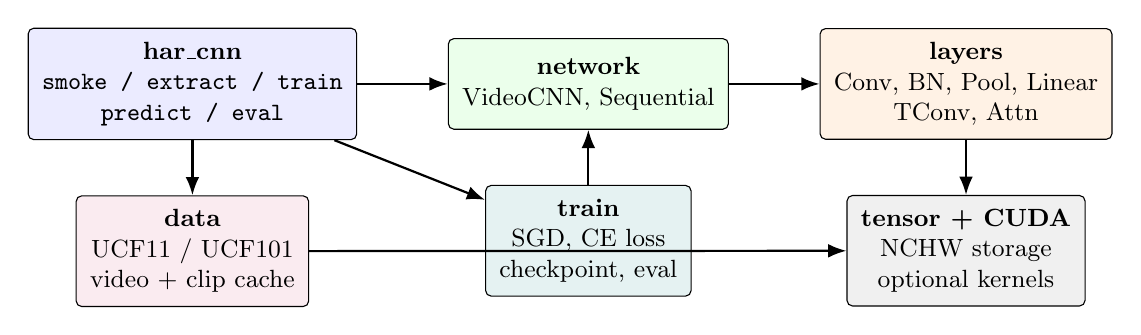
\begin{tikzpicture}[
  font=\small,
  box/.style={draw, rounded corners=2pt, align=center, inner sep=5pt,
              minimum height=1.15cm},
  arr/.style={-{Latex}, thick}
]
\node[box, fill=blue!8] (cli) {\textbf{har\_cnn}\\\texttt{smoke / extract / train}\\\texttt{predict / eval}};
\node[box, fill=green!8, right=1.15cm of cli] (net) {\textbf{network}\\VideoCNN, Sequential};
\node[box, fill=orange!10, right=1.15cm of net] (lay) {\textbf{layers}\\Conv, BN, Pool, Linear\\TConv, Attn};
\node[box, fill=purple!8, below=0.7cm of cli] (data) {\textbf{data}\\UCF11 / UCF101\\video + clip cache};
\node[box, fill=teal!10, below=0.7cm of net] (train) {\textbf{train}\\SGD, CE loss\\checkpoint, eval};
\node[box, fill=gray!12, below=0.7cm of lay] (ten) {\textbf{tensor + CUDA}\\NCHW storage\\optional kernels};
\draw[arr] (cli) -- (net);
\draw[arr] (net) -- (lay);
\draw[arr] (cli) -- (data);
\draw[arr] (cli) -- (train);
\draw[arr] (train) -- (net);
\draw[arr] (lay) -- (ten);
\draw[arr] (data) -- (ten);
\end{tikzpicture}
\caption{Main modules of AMSC-HAR. Almost all logic lives in headers under
\texttt{include/har/}.}
\label{fig:repo}
\end{figure}

\subsection{Build system}

CMake~3.25+ builds a C++23 target \texttt{har\_cnn}.
Two options control optional backends:
\begin{itemize}
  \item \texttt{HAR\_WITH\_OPENCV} (default ON): decode with OpenCV
        \texttt{videoio}; otherwise the code shells out to FFmpeg and
        writes temporary PNGs.
  \item \texttt{HAR\_WITH\_CUDA} (default ON): if \texttt{nvcc} is found,
        \texttt{src/cuda\_ops.cu} is compiled with
        \texttt{CMAKE\_CUDA\_ARCHITECTURES=86-real} (Ampere cubin only,
        avoiding PTX JIT mismatches between toolkit and driver).
\end{itemize}
Release builds use \texttt{-O3}.
On Windows, OpenCV DLLs are copied next to the executable after linking.

\subsection{Command-line interface}

Table~\ref{tab:cli} lists the subcommands implemented in \texttt{main.cpp}.

\begin{table}[t]
\centering
\caption{CLI of \texttt{har\_cnn}.}
\label{tab:cli}
\small
\begin{tabular}{@{}llp{8.4cm}@{}}
\toprule
Command & Typical use & Notes \\
\midrule
\texttt{smoke}   & sanity check & Tiny Conv-ReLU-Pool-Linear on synthetic $16\times16$ images; expects loss drop and $\ge 80\%$ acc. \\
\texttt{extract} & debug decoder & Writes resized frames from one video. \\
\texttt{train}   & fit VideoCNN  & UCF11 or UCF101; SGD, LR schedule, clip cache, \texttt{--resume}. \\
\texttt{predict} & folder demo   & Recursive video listing, top-$K$ softmax, optional folder-name labels. \\
\texttt{eval}    & split metric  & Loads a \texttt{.harw} file and scores train/val/test with per-class accuracy. \\
\bottomrule
\end{tabular}
\end{table}

A typical UCF11 training invocation is
\begin{lstlisting}
har_cnn train --dataset ucf11 --data data/UCF11_updated_mpg
              --size 64 --frames 8 --epochs 10 --batch 32
\end{lstlisting}
Inference on a folder of clips (used in Section~\ref{sec:exp}) is
\begin{lstlisting}
har_cnn predict --dir checkAcc --weights models/ucf11_videocnnBest.harw --top 3
\end{lstlisting}

\subsection{Checkpoint format}

Weights are stored as little-endian binaries with magic
\texttt{HARW001}.
The header records $H{=}W$, $T$, input channels, $K$, and the class-name
strings; then every tensor from \texttt{VideoCNN::state\_tensors()}
(learnable parameters plus BatchNorm running statistics) is dumped with
rank and shape.
This makes a checkpoint self-describing: \texttt{predict} rebuilds the
network from metadata instead of hard-coding $64\times 8\times 11$.

Decoded clips use a sibling format \texttt{HARF002} in
\texttt{data/ucf11\_cache/}, keyed by a hash of path and geometry, so the
expensive MPEG decode happens once.

%----------------------------------------------------------------------
\section{Tensor library and layers}
\label{sec:tensor}

\subsection{Tensors}

\texttt{har::Tensor<T>} is a dense, row-major, contiguous array with an
explicit shape and computed strides.
Images and activations use NCHW layout, which matches both the CPU
convolution loops and the CUDA kernels.
Allocation is either \texttt{new T[n]} on the host or
\texttt{cudaMallocManaged} when the default device is CUDA.
Elementwise arithmetic, \texttt{reshape}/\texttt{reshaped}, and
\texttt{sync()} (a device-wide barrier when CUDA is active) are provided
in the header.

A \texttt{Parameter<T>} pairs a data tensor with a same-shaped gradient
and a \texttt{requires\_grad} flag.
SGD and checkpointing iterate parameter lists; BatchNorm additionally
exposes non-parameter running mean/variance in the state dict.

\subsection{Layer contract}

Every spatial layer implements
\begin{align*}
  y &= f(x;\theta), &
  g_x &= \frac{\partial L}{\partial x}
       = \Bigl(\frac{\partial y}{\partial x}\Bigr)^{\!\!\top} g_y,
\end{align*}
by caching $x$ (and any auxiliaries) during \texttt{forward} and using
them in \texttt{backward}.
There is no tape interpreter: the graph is the C++ call stack of
\texttt{VideoCNN::forward} / \texttt{backward}.
This is easy to debug and maps one-to-one onto the kernels in
\texttt{cuda\_ops.cu}.

\subsection{Spatial operators}

\paragraph{Conv2D.}
A $K_h\times K_w$ kernel with stride $(s_h,s_w)$ and padding $(p_h,p_w)$
implements
\[
  y_{n,c',h',w'}
  = b_{c'} + \sum_{c,i,j} W_{c',c,i,j}\,
    x_{n,c,\,s_h h'+i-p_h,\,s_w w'+j-p_w}.
\]
Weights use a simple scaled-uniform init.
The CPU path is a direct 7-loop implementation; the CUDA path launches
\texttt{conv2d\_forward}/\texttt{conv2d\_backward}.

\paragraph{BatchNorm2D.}
Channel statistics are computed over $N\cdot H\cdot W$.
In training,
\[
  \hat x_c = \frac{x_c-\mu_c}{\sqrt{\sigma_c^2+\varepsilon}},\qquad
  y_c = \gamma_c\hat x_c + \beta_c,
\]
and $(\mu,\sigma^2)$ are written into exponential moving averages
(momentum $0.1$).
Eval uses the running statistics stored in the checkpoint, which is
essential for the 80\% folder test in Section~\ref{sec:exp}.

\paragraph{Pooling and activations.}
$2\times 2$ max-pool records argmax indices for the backward pass.
Global average pool collapses $H\times W$ to a 256-D frame embedding.
ReLU is $y=\max(x,0)$.
Dropout ($p=0.3$) is applied only on the pooled vector, and only in
training.

\paragraph{Linear and loss.}
The head is $z = W h + b$ with $W\in\mathbb{R}^{K\times 256}$.
Cross-entropy is the stable softmax + NLL
\[
  \ell = -\frac{1}{N}\sum_{n=1}^{N}\log
  \frac{e^{z_{n,y_n}-\max_k z_{n,k}}}
       {\sum_{j} e^{z_{n,j}-\max_k z_{n,k}}}.
\]
The backward gradient is $(\mathrm{softmax}(z)-e_y)/N$, moved back to the
activation device.

\subsection{Optimiser}

SGD with momentum $m=0.9$ and weight decay $\lambda=10^{-4}$ updates
\[
  v \leftarrow m v + (g + \lambda \theta),\qquad
  \theta \leftarrow \theta - \eta v.
\]
The learning rate starts at $\eta=3\cdot 10^{-3}$ and is multiplied by
$\gamma=0.5$ every 4 epochs (\texttt{--lr-step}).
Velocity buffers are allocated lazily to match parameter shapes and
devices.

%----------------------------------------------------------------------
\section{VideoCNN architecture}
\label{sec:model}

\subsection{Forward pass}

Let a batch of clips be $X\in\mathbb{R}^{N\times T\times 3\times H\times W}$
with default $H=W=64$ and $T=8$.
Time is flattened to a 2D batch of $NT$ frames.
A four-stage backbone produces a 256-D vector per frame; a temporal
residual block mixes neighbouring frames; attention pools time; a linear
layer outputs $K$ logits (Figure~\ref{fig:cnn}).

\begin{figure}[t]
\centering
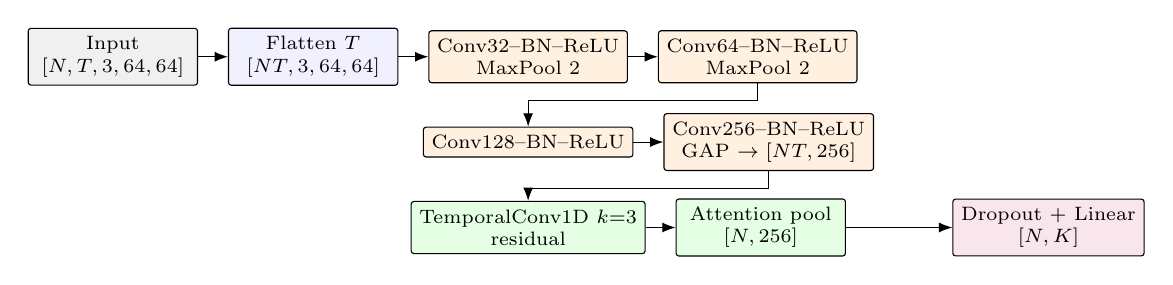
\begin{tikzpicture}[
  font=\scriptsize,
  node distance=0.38cm,
  blk/.style={draw, rounded corners=1pt, align=center, inner sep=3pt,
              minimum width=2.15cm, fill=blue!6},
  dim/.style={font=\tiny\ttfamily, text=black!55}
]
\node[blk, fill=gray!12] (in) {Input\\$[N,T,3,64,64]$};
\node[blk, right=of in] (flat) {Flatten $T$\\$[NT,3,64,64]$};
\node[blk, right=of flat, fill=orange!12] (c1) {Conv32--BN--ReLU\\MaxPool $2$};
\node[blk, right=of c1, fill=orange!12] (c2) {Conv64--BN--ReLU\\MaxPool $2$};
\node[blk, below=0.55cm of c1, fill=orange!12] (c3) {Conv128--BN--ReLU};
\node[blk, right=of c3, fill=orange!12] (c4) {Conv256--BN--ReLU\\GAP $\to[NT,256]$};
\node[blk, below=0.55cm of c3, fill=green!10] (tc) {TemporalConv1D $k{=}3$\\residual};
\node[blk, right=of tc, fill=green!10] (at) {Attention pool\\$[N,256]$};
\node[blk, right=1.35cm of at, fill=purple!10] (hd) {Dropout + Linear\\$[N,K]$};
\draw[-{Latex}] (in) -- (flat);
\draw[-{Latex}] (flat) -- (c1);
\draw[-{Latex}] (c1) -- (c2);
\draw[-{Latex}] (c2.south) -- ++(0,-0.22) -| (c3);
\draw[-{Latex}] (c3) -- (c4);
\draw[-{Latex}] (c4.south) -- ++(0,-0.22) -| (tc);
\draw[-{Latex}] (tc) -- (at);
\draw[-{Latex}] (at) -- (hd);
\end{tikzpicture}
\caption{VideoCNN data path. Spatial stages are shared across time; the
temporal block is residual ($h + \mathrm{TConv}(h)$).}
\label{fig:cnn}
\end{figure}

Spatial spatial sizes after padding-1 $3\times 3$ convolutions:
$64\!\to\!32$ (pool), $32\!\to\!16$ (pool), then $16\times 16$ until GAP.
Because image size must be divisible by 4, \texttt{build\_video\_cnn}
rejects illegal \texttt{--size} values.

\subsection{Temporal convolution and attention}

TemporalConv1D treats the $NT$ frame embeddings as $N$ sequences of length
$T$ and applies a depth-preserving 1D convolution of kernel size 3 with
zero-pad $1$:
\[
  u_{n,t,c'}
  = b_{c'} + \sum_{c=1}^{256}\sum_{k=-1}^{1}
    W_{c',c,k}\, h_{n,\,\mathrm{clamp}(t+k),\,c}.
\]
The residual $h+u$ lets the network keep a pure per-frame representation
when the temporal kernel is not yet useful.

Temporal attention pooling scores each time step with a learned query
$w\in\mathbb{R}^{256}$ (zero-initialised, so the first step equals a
temporal mean):
\begin{align}
  s_{n,t} &= h_{n,t}^{\top} w, &
  \alpha_{n,t} &= \frac{e^{s_{n,t}-\max_{t'}s_{n,t'}}}
                      {\sum_{t'} e^{s_{n,t'}-\max_{t''}s_{n,t''}}},
  \nonumber\\
  \bar h_n &= \sum_{t=1}^{T} \alpha_{n,t}\, h_{n,t}.
  \label{eq:attn}
\end{align}
The classifier then sees a single 256-D clip embedding.

\subsection{Capacity}

Table~\ref{tab:params} counts trainable tensors for $K=11$.
The last $3\times 3$ convolution and the temporal kernel dominate.
The released best file is $2\,361\,619$ bytes and contains 29 tensors
(parameters + four pairs of BN running stats), matching this layout
exactly.

\begin{table}[t]
\centering
\caption{Trainable parameter count of VideoCNN ($K=11$).}
\label{tab:params}
\small
\begin{tabular}{@{}lrr@{}}
\toprule
Block & Shape (main weights) & Parameters \\
\midrule
Conv $3\to32$ + BN            & $[32,3,3,3]$     & $960$ \\
Conv $32\to64$ + BN           & $[64,32,3,3]$    & $18\,624$ \\
Conv $64\to128$ + BN          & $[128,64,3,3]$   & $74\,112$ \\
Conv $128\to256$ + BN         & $[256,128,3,3]$  & $295\,680$ \\
TemporalConv1D                & $[256,256,3]$    & $196\,864$ \\
Attention query               & $[256]$          & $256$ \\
Linear $256\to 11$            & $[11,256]$       & $2\,827$ \\
\midrule
Total                         &                  & $\mathbf{589\,323}$ \\
\bottomrule
\end{tabular}
\end{table}

A smaller historical checkpoint
(\texttt{ucf11\_videocnn.64x8.harw}, $\approx 0.58$\,MB) corresponds to an
earlier narrower backbone.
A $112\times 16$ variant exists for higher-resolution experiments, at a
much larger activation cost.

%----------------------------------------------------------------------
\section{Data pipeline}
\label{sec:data}

\subsection{Decoding}

\texttt{extract\_video\_frames} opens a file with OpenCV
(\texttt{CAP\_FFMPEG}, then Media Foundation, then \texttt{CAP\_ANY}) or
with FFmpeg.
Frames are resized to $H\times W$, converted to RGB, scaled to
$[0,1]$, and stored as $[F,C,H,W]$ on the CPU.
When \texttt{uniform=true} (the dataset default), $F$ indices are spaced
over the reported frame count so a long YouTube clip is summarised rather
than truncated at the beginning.

UCF11 lives in a two-level tree
\texttt{<class>/<group>/video.mpg}.
The dataset walker skips annotation folders, sorts class names, and
assigns integer labels in that order---the same order written into
\texttt{.harw} class names.

\subsection{Cache and model clip}

To avoid re-decoding MPEG on every epoch, the loader first extracts
\texttt{cache\_frames=16} uniformly sampled frames and writes a
\texttt{HARF002} blob.
\texttt{sample\_model\_clip} then reduces 16 frames to the model length
$T=8$:
\begin{itemize}
  \item \textbf{Eval / no augment:} uniform subsample
        $t_i = i(T_{\mathrm{in}}-1)/(T_{\mathrm{out}}-1)$.
  \item \textbf{Train:} a random contiguous crop of 8 frames out of 16,
        optional horizontal flip (probability $1/2$), and optional time
        reversal (probability $0.3$).
\end{itemize}
If a clip is shorter than $T$, the last frame is repeated
(\texttt{pad\_clip}).

\subsection{Prefetch}

\texttt{train\_one\_epoch} optionally launches
\texttt{std::async} to decode the next host batch while the current batch
is on the device.
\texttt{--workers 0} disables the extra thread.
The first batch of an epoch prints mean and standard deviation of the
stacked tensor; a near-zero warning catches a broken decoder.

%----------------------------------------------------------------------
\section{Training procedure}
\label{sec:train}

Figure~\ref{alg:train} is the loop in \texttt{train\_video\_cnn}.
Each epoch shuffles training indices, applies augmentation, computes
cross-entropy, back-propagates through VideoCNN, and steps SGD.
Validation (and, if \texttt{--target-acc} is set, the test split) is
evaluated without dropout or augmentation.
The checkpoint with the best monitored score is written to
\texttt{models/<dataset>\_videocnn.harw} and reloaded for the final test
printout.

\begin{figure}[t]
\centering
\fbox{\parbox{0.92\linewidth}{\small
\textbf{Algorithm 1} Train VideoCNN on a HAR dataset.\\[0.25em]
Build model; optionally \texttt{load\_checkpoint(resume)}.\\
\textbf{for} epoch $=1\ldots E$ \textbf{do}\\
\quad step-decay $\eta$ every \texttt{lr\_step} epochs.\\
\quad shuffle train indices; \textbf{for} each minibatch \textbf{do}\\
\quad\quad load clips with augmentation; stack to $[N,T,C,H,W]$.\\
\quad\quad $z\leftarrow \mathrm{VideoCNN}(X)$;
          $\ell\leftarrow \mathrm{CE}(z,y)$; backward; SGD.\\
\quad evaluate val (and test if a target accuracy is set).\\
\quad if score improved: \texttt{save\_checkpoint}.\\
Load best weights; report test accuracy.
}}
\caption{Training loop implemented in \texttt{trainer.hpp}.}
\label{alg:train}
\end{figure}

Default hyperparameters (Table~\ref{tab:hp}) are the values baked into
\texttt{main.cpp} for UCF11.
Batch size is further clipped by
\[
  N_{\max}
  = \Bigl\lfloor
      \frac{16\cdot 16\cdot 112\cdot 112}{T\cdot H\cdot W}
    \Bigr\rfloor,
\]
so $64\times 8$ may use 32, while $112\times 16$ is forced down to 16.

\begin{table}[t]
\centering
\caption{Default UCF11 training hyperparameters.}
\label{tab:hp}
\small
\begin{tabular}{@{}llll@{}}
\toprule
Symbol / flag & Value & Symbol / flag & Value \\
\midrule
\texttt{--size} / \texttt{--frames} & $64$ / $8$ & $\eta$ / momentum & $0.003$ / $0.9$ \\
\texttt{--batch} / workers          & $32$ / $8$  & $\lambda$ (wd)    & $10^{-4}$ \\
\texttt{--epochs}                   & $10$        & dropout           & $0.3$ \\
\texttt{--lr-step} / \texttt{--lr-gamma} & $4$ / $0.5$ & seed         & $42$ \\
val / test ratio                    & $0.1$ / $0.1$ & cache frames   & $16$ \\
\bottomrule
\end{tabular}
\end{table}

Resume is class-count checked but does not restore optimiser state:
it is a warm start of $\theta$, not a bit-exact continuation.
\texttt{eval} bypasses training entirely, rebuilds the net from
checkpoint metadata, and prints overall plus per-class accuracy on a
chosen split.

%----------------------------------------------------------------------
\section{CUDA backend}
\label{sec:cuda}

When \texttt{HAR\_HAS\_CUDA} is defined and a device is present,
\texttt{default\_device()} returns CUDA unless \texttt{HAR\_DEVICE=cpu}
is set.
\texttt{src/cuda\_ops.cu} provides:
\begin{itemize}
  \item elementwise add/sub/mul/div and scalar variants;
  \item GEMM and transpose used by Linear;
  \item Conv2D forward/backward, ReLU, Dropout, max-pool, GAP;
  \item BatchNorm2D with a small device scratch buffer;
  \item TemporalConv1D forward/backward.
\end{itemize}
Kernels use a 1-D grid with 256 threads.
Attention pooling currently stays on the host (it is $O(NTC)$ with
$C=256$, $T=8$, and is not the bottleneck compared with the last
$3\times 3$ convolution).

Unified Memory simplifies the C++ API---the same \texttt{data()} pointer
is valid on both sides---but it requires the activation cap of
Section~\ref{sec:train} and a matching driver/toolkit pair.
The CMake comment documents a real failure mode: PTX produced by CUDA
13.3 cannot JIT on a 13.2 driver, which is why the project ships
\texttt{86-real} cubin only.

The inference experiment in Section~\ref{sec:exp} ran on the CPU path
(OpenCV decoder, no \texttt{nvcc} in the MSYS2 build).
Numerical results therefore do not depend on GPU reductions.

%----------------------------------------------------------------------
\section{Experiments}
\label{sec:exp}

\subsection{Setup}

All numbers below use \texttt{models/ucf11\_videocnnBest.harw}.
Peeking the header yields
\texttt{image\_size=64}, \texttt{max\_frames=8},
\texttt{in\_channels=3}, \texttt{num\_classes=11}, and the class list of
Table~\ref{tab:ucf11}.
The tensor inventory (29 entries) matches current
\texttt{VideoCNN::state\_tensors()}.
Inference ran with the rebuilt \texttt{har\_cnn} (C++23, OpenCV 4.13,
CPU).

\subsection{Folder test on 10 random UCF11 clips}

Ten videos were drawn uniformly from the 1600-clip tree, copied into
\texttt{checkAcc/<class>/}, and classified with
\texttt{har\_cnn predict --top 3}.
Folder names supply the ground-truth label.
Table~\ref{tab:ten} reports every clip.

\begin{table}[t]
\centering
\caption{Top-1 predictions on 10 random UCF11 videos
(\texttt{ucf11\_videocnnBest.harw}).}
\label{tab:ten}
\small
\begin{tabular}{@{}lllrc@{}}
\toprule
Clip & Label & Top-1 & $p$ & \\
\midrule
\texttt{v\_shooting\_12\_03}  & basketball           & basketball           & $99.3\%$ & ok \\
\texttt{v\_shooting\_17\_01}  & basketball           & biking               & $58.1\%$ & miss \\
\texttt{v\_diving\_14\_03}    & diving               & diving               & $99.9\%$ & ok \\
\texttt{v\_diving\_25\_02}    & diving               & diving               & $99.2\%$ & ok \\
\texttt{v\_swing\_22\_03}     & swing                & swing                & $81.2\%$ & ok \\
\texttt{v\_tennis\_02\_03}    & tennis\_swing        & tennis\_swing        & $99.9\%$ & ok \\
\texttt{v\_tennis\_15\_02}    & tennis\_swing        & tennis\_swing        & $98.2\%$ & ok \\
\texttt{v\_spiking\_05\_01}   & volleyball\_spiking  & volleyball\_spiking  & $95.5\%$ & ok \\
\texttt{v\_walk\_dog\_08\_05} & walking              & walking              & $38.0\%$ & ok \\
\texttt{v\_walk\_dog\_10\_02} & walking              & biking               & $56.7\%$ & miss \\
\midrule
\multicolumn{4}{@{}l}{Accuracy} & $\mathbf{8/10\ (80\%)}$ \\
\bottomrule
\end{tabular}
\end{table}

The model is clearly usable: six clips exceed $95\%$ confidence on the
correct class, including both diving examples and both tennis swings.
The two errors are informative rather than random.
\texttt{v\_shooting\_17\_01} is basketball but the softmax put biking
first ($58\%$) and basketball third ($14\%$).
\texttt{v\_walk\_dog\_10\_02} is walking; biking won ($57\%$) while
walking remained a close second ($40\%$).
A third walking clip was correct but only by a thin margin versus
horse-riding ($38\%$ vs.\ $36\%$).
These confusions are consistent with YouTube HAR: handheld cameras,
similar outdoor backgrounds, and cyclic leg motion shared by walking,
biking, and riding.

\subsection{How to read the best checkpoint}

A sibling file \texttt{ucf11\_videocnn.best86.harw} records a training
run that reached about $86\%$ on the monitored split.
The \texttt{Best} file used here is the 256-channel architecture
($2.36$\,MB), not the older $0.58$\,MB 64$\times$8 snapshot.
Because UCF11's test split is a random $10\%$ hold-out, a full
\texttt{eval --split test} on $\approx 160$ clips is the proper
unbiased number; the 10-clip probe is a smoke test of the released
weights, not a substitute for that split.

\subsection{Smoke test and software correctness}

\texttt{har\_cnn smoke} trains a 4-filter Conv-ReLU-Pool-Linear net on
32 synthetic $16\times 16$ images (centre-on vs.\ centre-off) for 80
epochs.
Passing requires a strictly decreasing loss and at least $80\%$
in-batch accuracy.
This does not measure HAR quality, but it guards against silent breaks
in convolution, pooling, SGD, or the CUDA/CPU switch.

\subsection{Limitations}

\begin{itemize}
  \item \textbf{Resolution and length.} $64\times 8$ discards fine
        racquet / ball detail and long temporal structure.
  \item \textbf{No optical flow.} Appearance-only features struggle
        when motion, not texture, is the cue.
  \item \textbf{UCF101} is supported but was not the focus of the
        checkpoint evaluated here; 101-way classification with the same
        0.6M model is a harder regime.
  \item \textbf{Attention on CPU} and Unified Memory make the GPU path
        simpler than a production trainer (no cuDNN, no mixed precision).
\end{itemize}

%----------------------------------------------------------------------
\section{Conclusions}
\label{sec:conc}

AMSC-HAR shows that a course-scale C++ stack---tensors, layers, SGD,
video I/O, checkpoints, and optional CUDA---is enough to train and
deploy a real action classifier.
VideoCNN is small ($5.9\times 10^5$ parameters) and explicit: shared
2D features, residual temporal convolution, and attention pooling
(Eq.~\eqref{eq:attn}).
On UCF11 the released best weights recognise most held-out YouTube
clips with high confidence; a 10-video random probe scored $80\%$,
with residual errors concentrated on walking / biking / basketball.

Natural extensions are a full test-split table with per-class metrics,
optical-flow or two-stream fusion, a deeper temporal module, mixed-precision
CUDA, and a proper UCF101 run with the official split files.
The important property of the project is that each of those upgrades
would touch a few headers rather than a third-party graph compiler.

%----------------------------------------------------------------------
\begin{thebibliography}{9}

\bibitem{liu2009ucf11}
J.~Liu, J.~Luo, and M.~Shah,
``Recognizing realistic actions from videos `in the wild',''
in \emph{Proc.\ IEEE Conf.\ Computer Vision and Pattern Recognition (CVPR)},
2009.

\bibitem{soomro2012ucf101}
K.~Soomro, A.~R.~Zamir, and M.~Shah,
``UCF101: A dataset of 101 human actions classes from videos in the wild,''
CRCV-TR-12-01, University of Central Florida, 2012.

\bibitem{wang2013dt}
H.~Wang and C.~Schmid,
``Action recognition with improved trajectories,''
in \emph{Proc.\ IEEE Int.\ Conf.\ Computer Vision (ICCV)}, 2013.

\bibitem{simonyan2014twostream}
K.~Simonyan and A.~Zisserman,
``Two-stream convolutional networks for action recognition in videos,''
in \emph{Advances in Neural Information Processing Systems (NeurIPS)}, 2014.

\bibitem{tran2015c3d}
D.~Tran, L.~Bourdev, R.~Fergus, L.~Torresani, and M.~Paluri,
``Learning spatiotemporal features with 3D convolutional networks,''
in \emph{Proc.\ IEEE Int.\ Conf.\ Computer Vision (ICCV)}, 2015.

\bibitem{wang2016tsn}
L.~Wang, Y.~Xiong, Z.~Wang, Y.~Qiao, D.~Lin, X.~Tang, and L.~Van~Gool,
``Temporal segment networks: Towards good practices for deep action recognition,''
in \emph{Proc.\ European Conf.\ Computer Vision (ECCV)}, 2016.

\bibitem{carreira2017i3d}
J.~Carreira and A.~Zisserman,
``Quo vadis, action recognition? A new model and the Kinetics dataset,''
in \emph{Proc.\ IEEE Conf.\ Computer Vision and Pattern Recognition (CVPR)},
2017.

\end{thebibliography}

\end{document}
